\documentclass[12pt]{third-rep}

%% Any characters from a % to the end of line are comments.

%% The third-rep class and this starter kit were written by 
%% Graham Gough <graham@cs.man.ac.uk>
%% If you have any comments or questions regarding this document,
%% please post them to the local newsgroup man.cs.tex.

%% This skeleton report is organised as a master file called
%% report.tex which then includes files for individual parts including
%% abstract.tex, chapter1.tex, chapter2.tex, chapter3.tex and
%% appendix1.tex.  

%% The third-rep style is a locally created style based on the
%% standard LaTeX report style. If you really want to have a look at
%% it, its source can be found in
%% /usr/local/share/texmf/tex/latex/mancs/third-rep.cls
%%
%% More information about LaTeX in general and the local setup in
%% particular can be found on the web at 
%% http://csis.cs.manchester.ac.uk/software/contrib/latex
%%
%%%%%%%%%%%%%%%%%%%%%%%%%%%%%%%%%%%%%%%%%%%%%%%%%%%%%%%%%%%%%%%%%%%%%%%%
%%
%% This is an example of how you load extra packages.
%% Some packages are already loaded in the third-rep class

%%\usepackage{url} % typeset URL's sensibly

\usepackage{pslatex} % Use Postscript fonts

%% The best way to latex just one chapter is to uncomment lines such as
%% the next:
%\includeonly{chapter1}

%% This defines the title (the \\ forces a line break)
\title{Visualisation of Allergy\\
  Hotspots}
%% and author
\author{Nick Burrell}
%% and supervisor
\supervisor{Dr. Andy Carpenter}
%% and the year of the report
\reportyear{2017}

%% this defines the file that contains the text of the abstract, there
%% must be one of these by the time you submit your report.
\abstractfile{abstract.tex}

%% this defines the file that contains the acknowledgements (it can be
%% omitted if you don't feel like thanking anyone
\thanksfile{merci.tex}

%% Uncomment the following lines if you want to include the date as a
%% header in draft versions. See the documentation for fancyhdr for
%% more ways of modifying headers (texdoc fancyhdr will show you the
%% docs) 

\usepackage{fancyhdr}
\pagestyle{fancy}
\lhead{}  % left head
\chead{Draft: \today} % centre head
\lfoot{}
\cfoot{\thepage}
\rfoot{}

%% The following line sets up the use of PostScript fonts rather
%% than the standard bitmapped fonts.
\usepackage{pslatex}

%% Uncomment the following line if you want to change the name of the
%% Bibliography to References
%\renewcommand{\bibname}{References}

\usepackage{listings}

%% End of preamble, the actual document starts here
%%

\begin{document}

%% This actually creates the title and abstract pages
\dotitleandabstract

%% Generate contents etc
\tableofcontents
\listoffigures
\listoftables

%% These include the actual text
\chapter{Introduction}
\label{cha:intro}

I will briefly explain my motivation for this project, my initial aims also provide an overview of what you will read in this report.

\section{Motivation} 
I have a long history with allergies. As far back as I can remember I have suffered from allergy symptoms ranging from waking up with gummy eyes to having a permanently sealed nose and tight chest. I've had little luck with medication so I usually end up trying to change my environment to limit the number of allergens with an air filter. Even an industrial air filter does not provide much relief for me.\\

When I saw this project proposed by Dr Markel Vigo I knew it was for me. The challenge of trying to find potential causes for specific allergies was quite exciting. Not only would providing a means for identifying hotspots and their causes help the scientific community, it would also help me personally.\\

The majority of my previous programming experience has been with java within the school and C\# when working for companies outside of University. I quickly realised this project would have to be done using some kind of web technology, so the fact I had very little experience with this side of computer science, I decided it'd be a great opportunity to develop my skill sets to help my career.\\

\section{Aim}
\label{sec:aim}

I gave myself the following four main goals that I wanted Inhale to fulfil;

\begin{enumerate}
  \item Visualise hotspots
  \item Be user friendly
  \item Be useful for future users. Both general public and researchers.
  \item Be accessible
\end{enumerate}


The most emphasis was on the identification of allergy hotspots. I wanted a hotspot algorithm that was both valid and  powerful to be combined with a useful visualisation technique. As I want Inhale to be useful for the general public, it's important that the visualisation technique used both looks good and accurately displays the hotspots generated by the algorithm.\\

%% Before anything data related, explain hotspots

\section{Report Overview}

There are no hard to understand, advanced computer science algorithms or techniques used in this project. However, I do make some decisions that will require some background knowledge and context of the related subjects in order to fully understand my reasoning. So the second chapter will provide a brief history of allergies and how certain types of allergies are relevant to my project.\\

I'll talk about the structure and content of the datasets used throughout and cover what similar applications already exist.\\

Once the basics are understood, I will take the reader through the design decisions and implementation stages of Inhale in Chapters 3 and 4. I will go into some detail of the core processes, but nothing too heavy.\\

Chapter 5 will explain how I did my testing and how I interpreted the resulting heatmap displayed by Inhale. I'll show you some of the interesting hotspots and how I evaluated them.\\

I'll conclude the report with a summary of my personal experience developing Inhale and my findings using the final product.\\
    

\section{Software Environment}

My environment options for Inhale were to make a Desktop Application for either Windows or MacOS, website, mobile app or a web application.\\

I decided against making a desktop app for any platform as by going with this route it limits the number of users instantly. Whilst the last two versions of Windows make up around 65\% of the Desktop market, that's still a potential 35\% of users that are completely unable to use my software \cite{windows}. As this project is likely to be shown to potential employers, it would be nice to have it on a platform that is easier to setup and get running.\\

A mobile application was a strong contender, with 

\subsection{Occam}

Here is some more example text, showing various \LaTeX\ facilities
you may need.  The project was mostly programmed in
\textbf{Occam}~\cite{occam}.  (A citation has been created  here to an
entry in the bibliography at the end of the report. See
chapter~\ref{cha:bib} for more details on how to do this).

Note the way of getting boldface, \textit{textit} is used for italic.
\emph{emph} is used for emphasis and is the same as italic except when
already in italic.  Note the cross reference to the bibliography.
This is how you create a footnote: DMA\footnote{Direct Memory Access.
  Footnotes can stretch over more than one line if you have a lot to
  say, but be careful not to overdo them.}.

Here is a reference to a figure. See figure~\ref{pipeline}.
\begin{figure}[htbp]
  \centering
  \setlength{\unitlength}{0.0125in}
\begin{picture}(300,35)(60,730)
\thicklines
\put(340,750){\vector( 1, 0){ 20}}
\put( 80,740){\framebox(20,20){}}
\put( 60,750){\vector( 1, 0){ 20}}
\put(100,750){\vector( 1, 0){ 20}}
\put(120,740){\framebox(20,20){}}
\put(180,750){\vector( 1, 0){ 20}}
\put(200,740){\framebox(20,20){}}
\put(160,740){\framebox(20,20){}}
\put(140,750){\vector( 1, 0){ 20}}
\put(240,740){\framebox(20,20){}}
\put(220,750){\vector( 1, 0){ 20}}
\put(260,750){\vector( 1, 0){ 20}}
\put(280,740){\framebox(20,20){}}
\put(320,740){\framebox(20,20){}}
\put(300,750){\vector( 1, 0){ 20}}
\end{picture}

  \caption{A Pipeline of processors
    \label{pipeline}}           %  this label must appear after the
                                %  \caption, and before the end of the
                                %  figure
\end{figure}
The picture in this figure was created the hard way using the picture
facility of \LaTeX. It is \emph{much} easier to use \texttt{xfig}, as
described in section~\ref{sec:diagrams}.  Whatever its contents, a
figure `floats' to a `suitable' point in the text and is never split
across a page boundary. (\LaTeX's idea of what constitutes a suitable
point may not coincide with yours)


Now we have a verbatim environment; this is a useful way of including
snippits of program, printed in a fixed width font exactly as typed:

\begin{verbatim}
{{{ An example of some folds
...  This is some folded code
  {{{ This is another fold
  This is text within the fold that has now been
  opened so that the text can be read.
  }}}
}}}
\end{verbatim}

% Everything below here is commented material which is used by the
% emacs tex support system called auctex. If you're not an emacs user
% you can safely ignore it. If you do use emacs you should take a look
% at the local emacs or LaTeX WWW pages for more on emacs support for
% LaTeX.

% Local Variables:
% mode: latex
% TeX-master: "report"
% End:


\chapter{Background}
\label{cha:back}

In this chapter I will cover the context of my project to allow the reader to understand the more complex parts of the report to come. First I will explain the different symptoms of hay fever and how they might be caused by different allergens. I will then talk about the main dataset used throughout and how I interpreted the data to produce meaningful results.

\section{Seasonal Allergies}
A massive 44\% of Britons suffer from at least one allergy, the majority suffering from some form of a seasonal allergy \cite{mintelallergy}. Allergies are on the rise, even with modern allergy medication continuously improving \cite{mintelallergy}. It is clear that something needs to be done to help those who suffer.\\


\subsection{Asthma}
When talking about hay fever, most people assume that it only affects the nose. However, in a study by Eur Respir J, it was found that 20.4\% of allergy sufferers also self-reported suffering from asthma \cite{rhinitis}. By 2025, it is predicated that asthma will represent the most prevalent chronic childhood disease and result in one of the highest health care costs, primarily due to the need for ongoing treatment throughout the patients life \cite{childhood}. Despite many decades of research, we do not have a complete working solution to the problem. The best we can do is limit exposure, Inhale will help with this by highlighting areas with unusually high occurrences of particular symptoms.\\

Listed below are the main causes of allergy induced asthma, the effects of which can impact everyday life of the sufferer.\\


\begin{itemize}
  \item Allergens: including pollen, dust mites, animal fur ("dander") or feathers
  \item Airborne Irritants: including cigarette smoke, fumes and pollution
  \item Emotions: including stress or laughter
  \item Weather Conditions: including sudden changes in temperature, cold air, windy days, thunderstorms and hot, humid days
  \item Infections: particularly infections of the upper airways, such as colds and flu
\end{itemize}\begin{center}Adapted from \cite{urlasthmacauses}\end{center}

There is a large variety of factors contributing to allergy induced asthma. It would be impossible to cover all aspects of these in this report. I am going to focus on the effects of Airborne Irritants and Allergens.


\section{Datasets}

In this section, I will describe the structure and features of the datasets used by Inhale.\\

\subsection{Britain Breathing}

Britain Breathing is a Citizen Science project run by the British Society for Immunology, Royal Society of Biology and the University of Manchester Immunology Group, who conduct research into the causes and treatment of allergies. To aid their research, they collect data on seasonal allergies using a simple but effective mobile application available on the Android operating system. Their aim is to get allergy sufferers to submit their symptoms regularly so that they can build solutions to the problem.\\

When setting up the application, you are asked standard registration questions such as your age, gender, and whether you suffer from pre-existing allergy related issues such as asthma and hay fever. In everyday use of the Britain Breathing app you are asked to rate the severity of your allergy related symptoms on each day. You are also asked whether you have taken your allergy medication for that day. This data is collected along with your location to be stored by Britain Breathing.

\begin{figure}[H]
\begin{center}
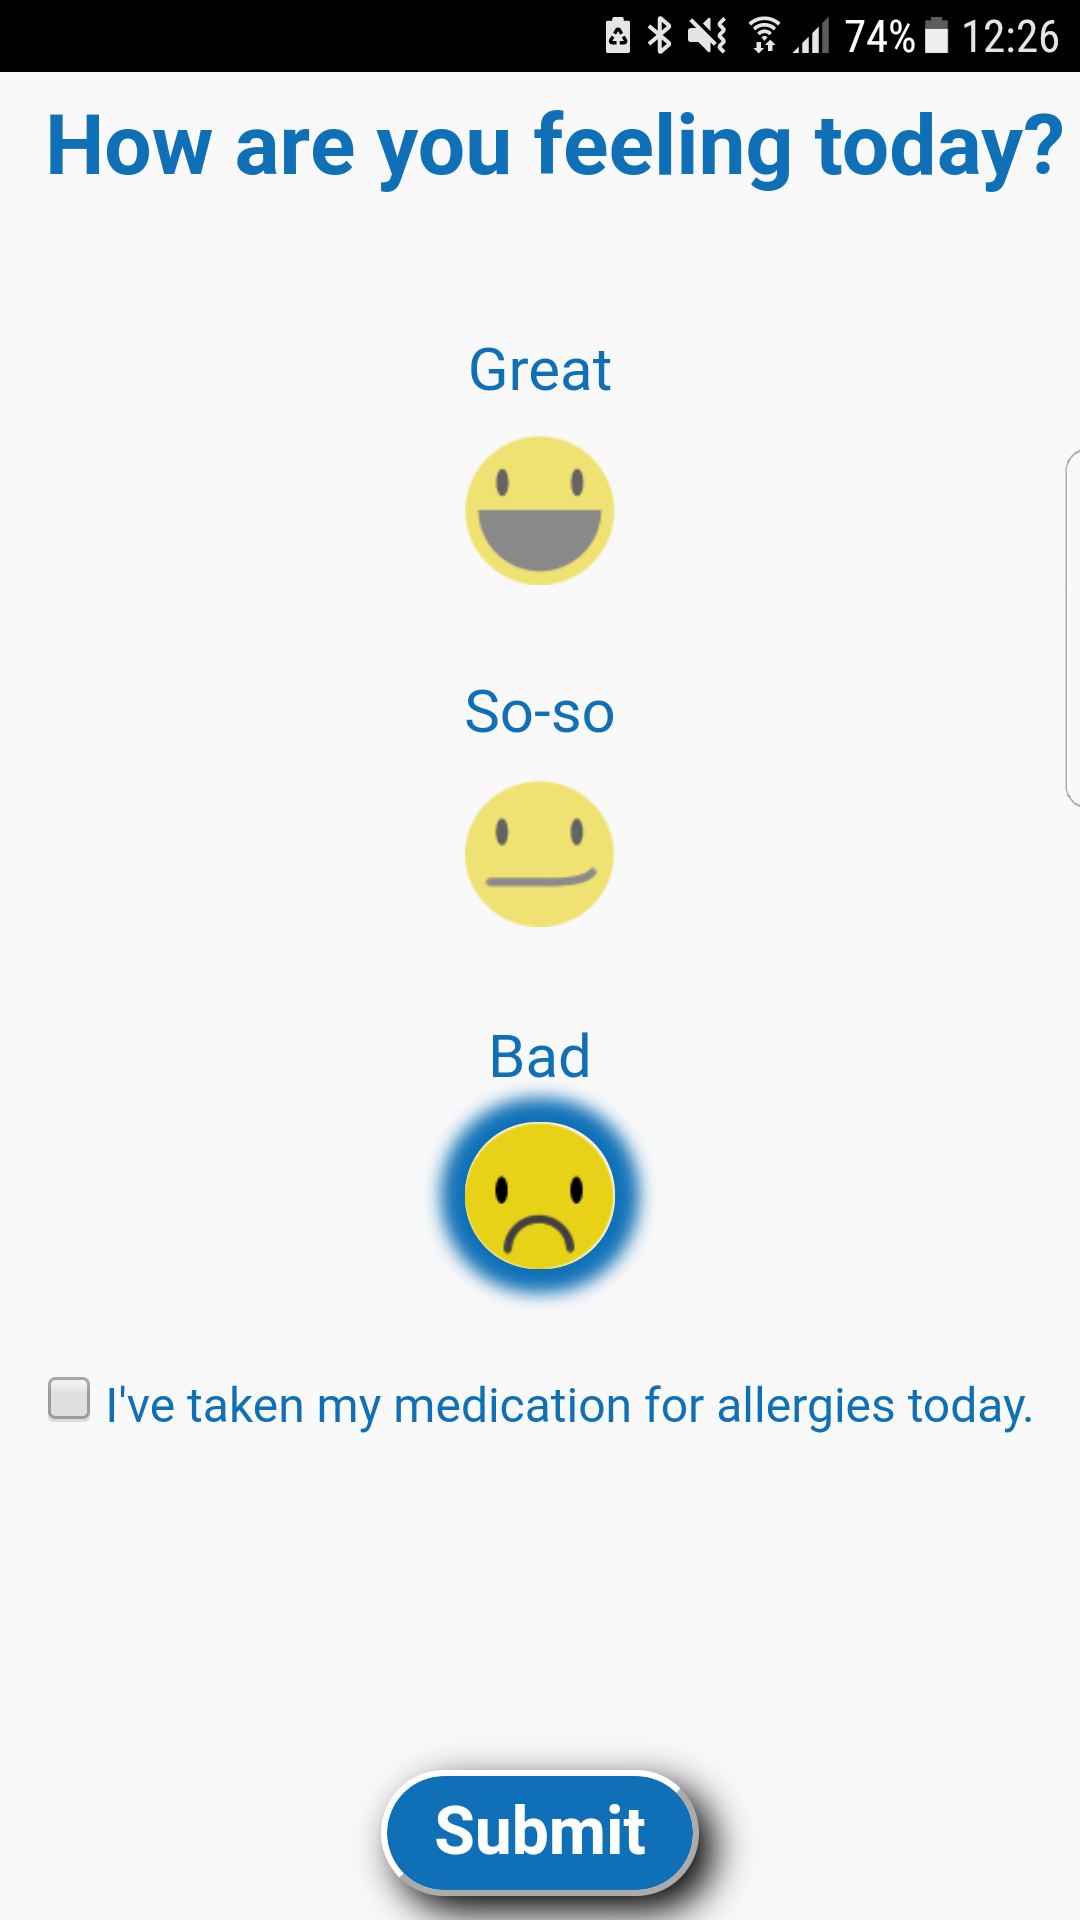
\includegraphics[width=6cm, height=8cm]{bbapp}
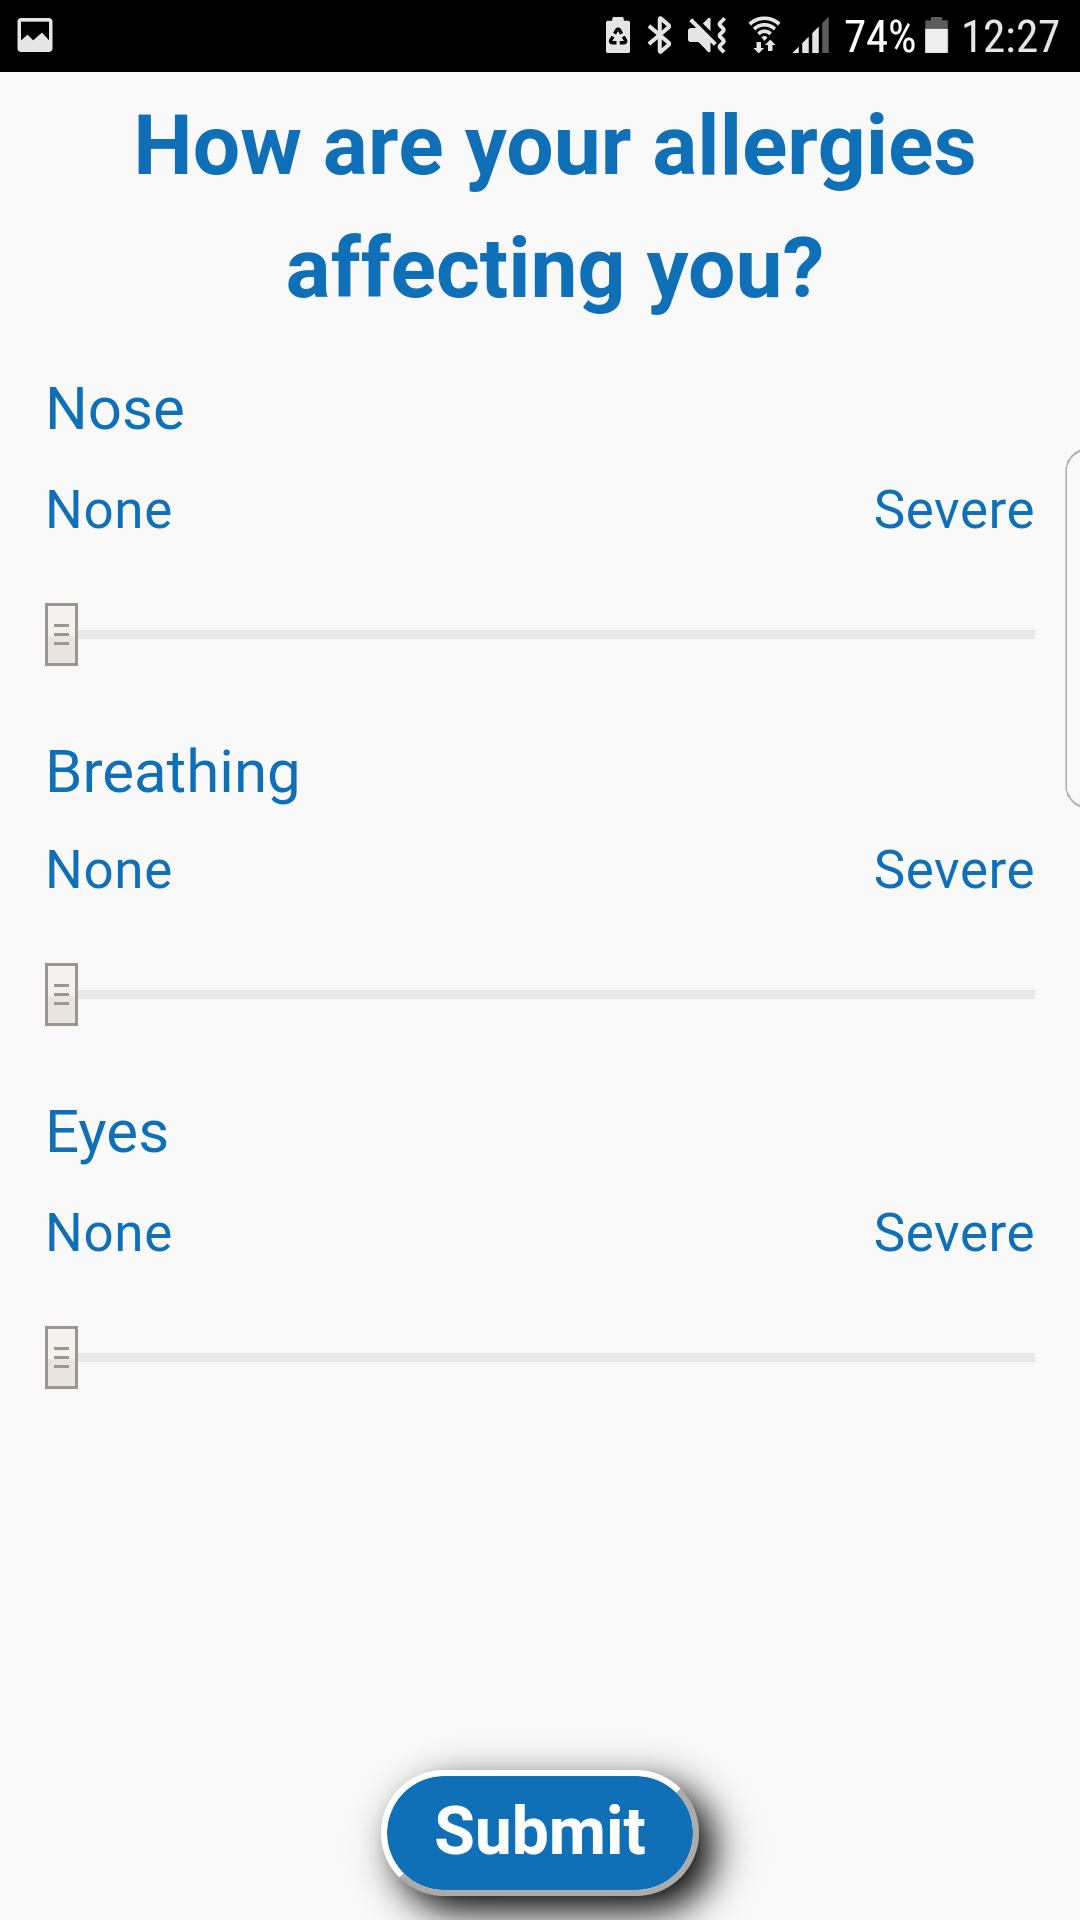
\includegraphics[width=6cm, height=8cm]{bbapp2}
\caption{Screenshots of the data collection screen on the Britain Breathing Android app}
\label{fig:bbscrn}
\end{center}
\end{figure}

Dr Vigo works with the Britain Breathing project, and was kind enough to provide me with their dataset from September 2016. This dataset contains 18,386 records from all over the UK. The data contains values corresponding to the questions asked in the application. They also ask whether or not the user has taken their medication today, this field is particularly useful as it can be used as a multiplier. If someone has severe nose, eye and breathing symptoms and they have taken their medication, then this should be expressed in the final visualisation as they're clearly being exposed to a significant amount of allergens.\\% avoid 'obviously', rephrase

The dataset covers nose, eye and breathing symptoms, see Table \ref{bbdatatable}. As these parts of the body are all interlinked in very close proximity, it makes sense to try to combine them. In Section \ref{sec:anal}, I will go into more detail as to how I combine these problematic areas into one value that summarises them.\\


\begin{table}[H]
\begin{center}
\begin{tabular}{|c|c|c|c|c|c|c|c|c|c}\hline\hline
Breathing&Eyes&How Feeling&Nose&Taken Meds&Asthma&Hay Fever&Latitude&Longitude\\\hline
0&0&0&0&1&1&0&54.10&-2.39\\
3&0&2&3&1&1&1&53.89&-2.79\\
3&1&0&3&1&1&1&53.24&-2.34\\\hline\hline
\end{tabular}
\end{center}
\caption{A Simplified sample of the 18,386 record Britain Breathing dataset}
\label{bbdatatable}
\end{table}

The Britain Breathing dataset will be the base for the entire project. Most of my time was spent with this set establishing a good hotspot identification algorithm and presenting it on a map.

\subsection{Other Datasets}

Whilst early testing and development involved many datasets, I decided on two main sets to use for comparison to the Britain Breathing dataset.\\

The data.gov website provides counts for Road Traffic data available for public use. The set contains 750,000 entries from major road traffic counts at locations all over the UK. They give a location of the Centre Point of the count, that is, where the counter was when recording the traffic. The northmost and southmost junctions on either side of the Centre Point. For each record, the counts for different vehicle types are given. Vehicles are categorised into Cars, Buses, Large Goods Vehicles (LGV), Heavy Goods Vehicle Rigid axle (HGVRx) and HGVAx for articulated HGV's where x is the number of axles of the HGV. See Table \ref{RoadTrafficData} for a simplified version of the dataset.\\


\begin{table}[H]
\begin{center}
\begin{tabular}{|c|c|c|c|c|c|c|c|c|c|c|}\hline\hline
S Ref E&S REF N&Road&A REF E&A REF N&Hour&CAR&BUS&LGV&HGVR2&...\\\hline
90200&10585&A3112&90320&10530&7&24&6&13&5&...\\
380927&405391&M60&382819&405920&15&7642&18&300&64&...\\
380927&405391&M60&382819&405920&17&10042&32&654&103&...\\\hline\hline
\end{tabular}
\caption{Simplified example of the 750,000 record Road Traffic dataset. 20 columns have been removed for viewing purposes.}\label{RoadTrafficData}
\end{center}
\end{table}

The second set used is a dataset of the large urban areas in the UK. The data is fairly simple consisting of a location feature in the form of a Latitude and Longitude and a name for the area. I used this dataset as a guide in the hope that it might help highlight interesting areas. Areas that are not in a large urban area but are indicated as a hotspot should be investigated further. However, it is not used for any particular research benefit, nor is it used to draw any conclusions.\\

\section{Using Datasets}

The number of people suffering from allergic rhinitis is rising, and whilst increased carbon emissions and global warming are lengthening the pollen season, there are not significantly more pollen producing plants and trees year on year \cite{co2pollen, allergyrising}.\\

The main pollutants emitted by combustion engine vehicles are:

\begin{itemize}
    \item CO
    \item $SO_2$
    \item $NO_x$
\end{itemize}

\begin{center}
Adapated from \cite{vehcemis}
\end{center}

It has been proven that these pollutants, whilst perhaps not associated with hay fever symptoms by most, are actually all directly associated with allergic rhinitis\cite{airPollution}. With this in mind, we can compare the Road Traffic dataset with the Britain Breathing dataset on the same map to try and find some correlation.\\

\section{Existing Applications}
\label{sec:diagrams}

There are few directly relevant applications. The reason for this is that in order to produce a meaningful application a well-formed dataset is required. In order for a dataset to be relevant, it needs to be of a reasonable size, have a good range of locations and a diverse demographic. Without collecting data from the people directly affected by allergens it's not possible to make educated conclusions on allergy hotspots. Currently there are no existing applications that satisfy this criteria.\\

\subsection{Britain Breathing}
Britain Breathing have a Data Visualiser on their website. It provides a simple display of the allergy data collected in a particular data range, for a particular data value. At the time of writing this report, the Visualiser is not working so I can only display a screenshot of the interface without the map containing the visualisation.

\begin{figure}[H]
\begin{center}
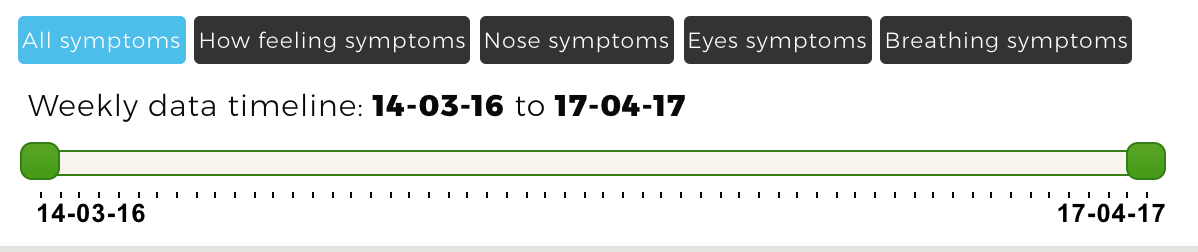
\includegraphics[width=0.75\textwidth]{bbvisinterface}
\caption{Britain Breathing Visualiser Interface}
\end{center}
\end{figure}

\subsection{Pollen forecast}

The most comparable applications to Inhale are pollen forecast services such as Pollen.com's allergy forecast map. As the name suggests it only displays pollen forecasts, not allergy symptoms. Whilst pollen is a major contributor to allergy symptoms, it needs to be combined with the other problematic allergens to be make credible conclusions.\\

Therefore, without the data from an organisation like Britain Breathing, it is not possible to make a comparable application.

\begin{figure}[H]
\begin{center}
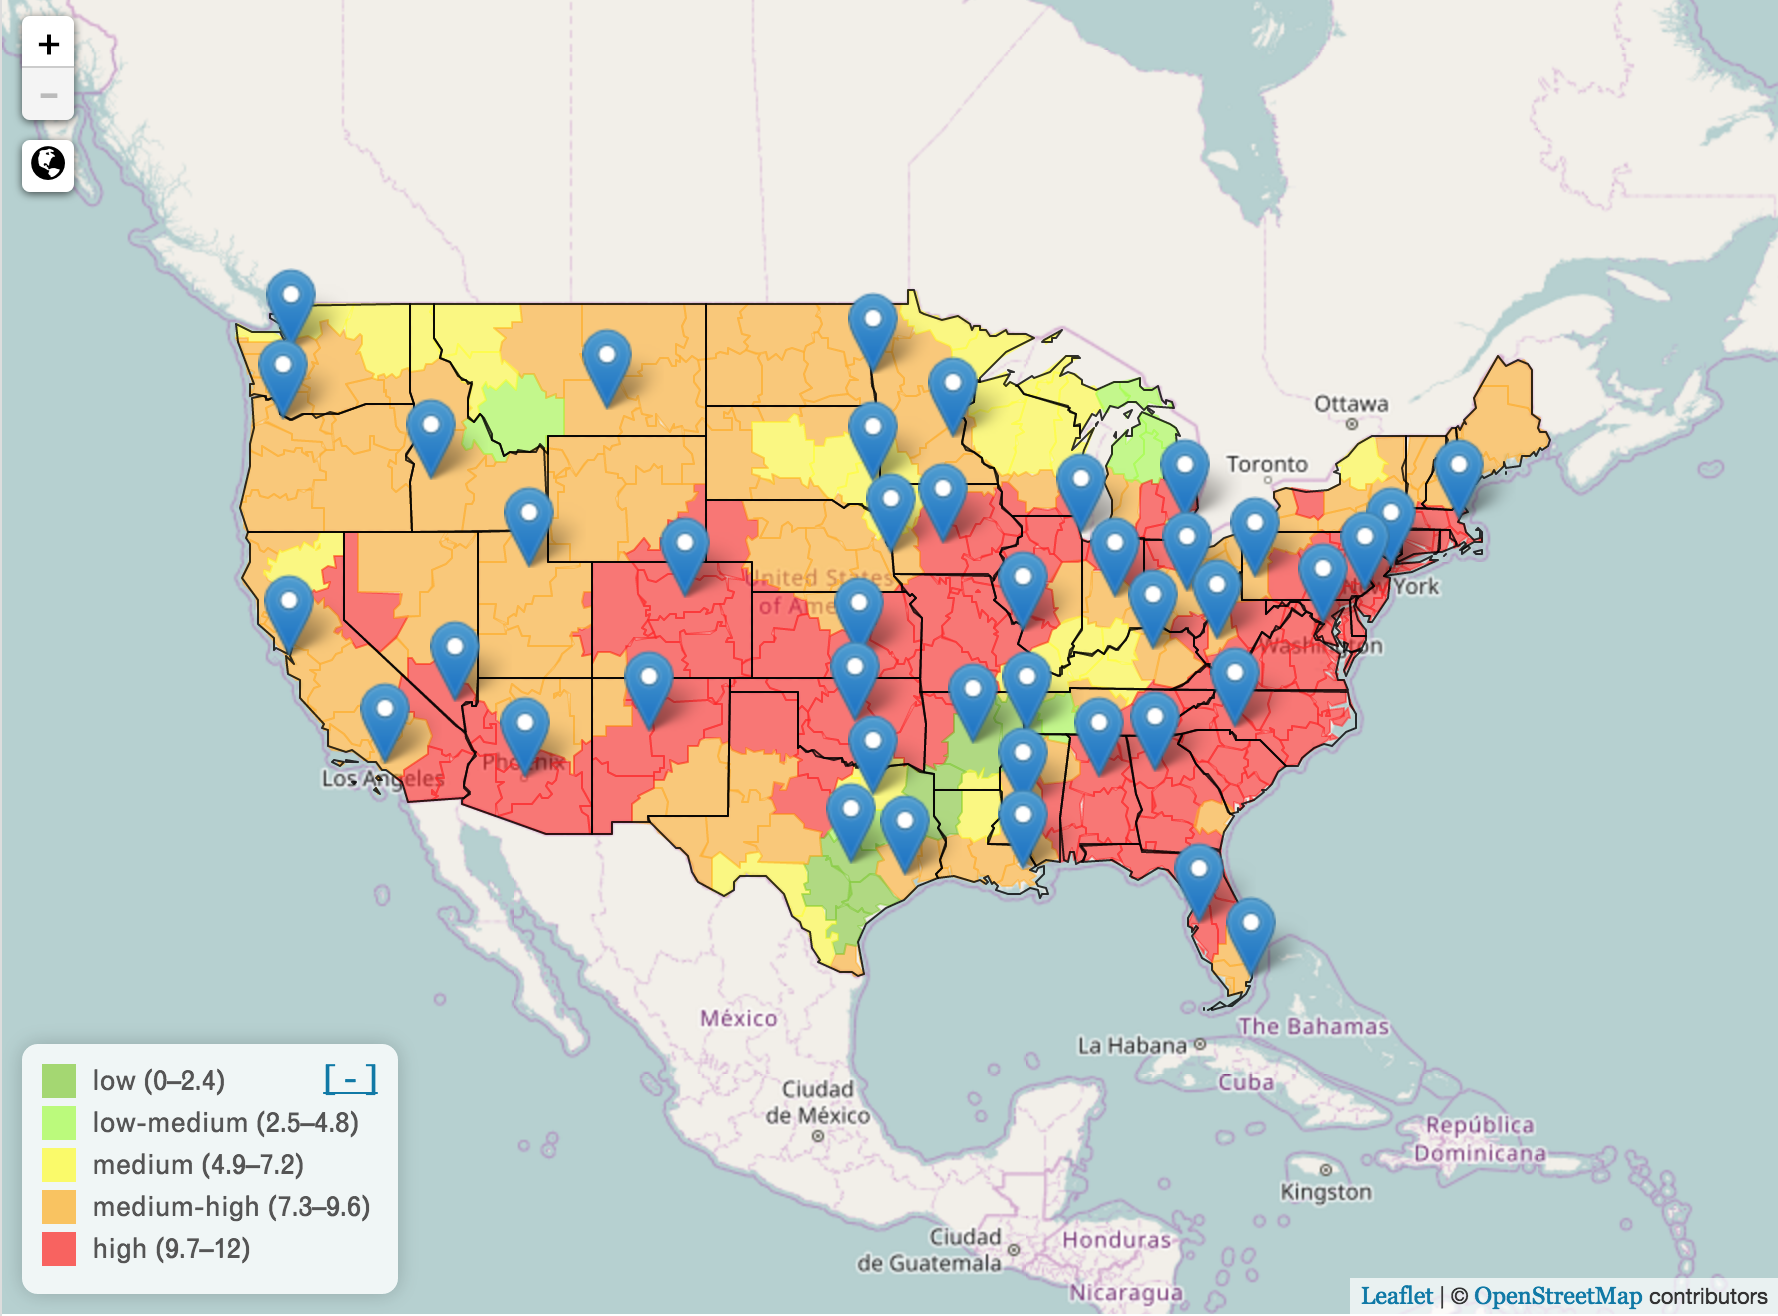
\includegraphics[width=0.75\textwidth]{pollenforecast}
\caption{Pollen.com Allergy Forecast Map}
\end{center}
\end{figure}

\section{Remarks}

After looking at many other mapping applications, it has become clear that using the standard Marker to represent points on a map can be used if and only if there are a very low density of points. Any other scenario results in a map that is totally incomprehensible.

\begin{figure}[H]
\centering

\includegraphics[width=0.05\textwidth]{marker}
\caption{Marker}\label{fig:marker}
\end{figure}
\chapter{Design}
In this Design section, I'll explain how and why I chose the Software Architecture I did, and what tools I used to develop Inhale. I won't go into the details, just enough so that the Design choices are justified.

\section{Architecture Choice}

As all of the datasets I'll be using for Inhale will be geographical datasets, meaning they all have a location attribute, it is imperative that they are displayed on a map. Trying to make any sense of a geographical dataset without seeing it on a familiar map is nearly impossible.\\



\subsection{ArcGIS by Esri}

ArcGIS is an incredibly powerful contextual tool for mapping and spatial reasoning. Its features are so well made that I initially thought using some form of this software would be the only viable solution. It allows you to produce good-looking, user-friendly maps with very few lines of code. It  also provides a mass of data processing tools, including hotspots analysis and data correlation.\\

Ultimately, I chose not to go with ArcGIS because it costs around £1200 for one license. However I also wanted to implement my own algorithms, using ArcGIS would not leave me with much to implement, and after all, this is a computer science project. I can see how ArcGIS could be incredibly useful for businesses and marketing/pr.

\subsection{Desktop Mapping Tools}

There are various desktop mapping tools available, even open source options that have a good variety of features. The main issue with this style of mapping software is it's expandability, accessibility and familiarity.\\

Although tools like MapSphere allow you to make 3rd party plugins to expand the standard application with your own features, the features you're given access to when developing those plugins is quite limited. I want the scope to be able to implement whatever I want. 
Being a desktop application, you're cutting down your potential users, not everyone wants to download an application, it feels too heavy and sluggish for modern users when you can access perfectly able maps from our pockets in the form of smartphone apps and websites. I wanted Inhale to be familiar to the user, I wanted to use controls people are used to using from their everyday use of Google Maps, Waze etc. All of the free desktop applications I tried felt very old and sluggish.\\

\subsection{Google Maps}

After playing around with ArcGIS and desktop mapping tools, I was aiming more towards a solution involving a dynamic mapping provider. Google Maps does not need an introduction. Google have an API that allows developers to implement their own features, toolbars and map tiles. The API can provide maps on various platforms from Android, iOS, javascript and more.\\

The biggest draw towards Google Maps is their places API, it allows you to search for establishments, geographic locations, or prominent points of interest in a well defined area around a point \cite{googlePlaces}. This would be incredibly useful for Inhale as once a hotspot is identified, you could search for nearby places that may be contributing to the symptoms in that area. The only problem here is that it's very difficult to implement a general approach to getting nearbly places that have an affect. Google sort their places by type, the types are aimed towards general public use. They're in categories such as art gallery, bakery, bank, pharmacy, hospital. Whilst it could be argued that you could count the number of commercial premises nearby, but I don't believe this is enough to provide any sort of answer to allergy hotspots.\\

Google Map's main downfall is the lack of customisability, it lacks some features compared to other mapping options.

If Google ever increase the number of categories, or maybe include more general options such as "industrial" or "factory" then it would definitely be the best option.\\

\subsection{Leaflet}

Leaflet is a javascript library for mobile-friendly interactive apps \cite{leaflet}. Leaflet is comparable to Google Maps in that it has many of the same features. Leaflet is open source, has many third party plugins with a thriving community contributing daily towards building a versatile dynamic mapping tool.\\

I decided to use Leaflet for my project as it is the most customisable of all the options investigated so far. It allows me to develop whatever I want to, and make my map look exactly how I want.\\

One particular third party plugin that drew me towards Leaflet was heatmap.js. Heatmaps seem like the best way to present the results of a hotspot identification algorithm. After testing the built-in Google Maps heatmap, I was disappointed with both the speed and custom options available.\\

Leaflet was chosen because it can be used in a web format, it is very customisable and it has a lively community contributing to features all the time. I would be easy to add necessary features further down the line.

\section{Leaflet}

Talk about how you use leaflet.

So, once the data is ready to be displayed, you pass to leaflet as heatmap layer.

Deals with layers

Tiles - Simplicity - familiarity

\section{Development Tools}

Tableau

Chrome dev tools

\bibliography{refs}             % this causes the references to be
                                % listed

\bibliographystyle{alpha}       % this determines the style in which
                                % the references are printed, other
                                % possible values are plain and abbrv
%% Appendices start here
\appendix
\chapter{Example of operation}

An appendix is just like any other chapter, except that it comes after
the appendix command in the master file.

One use of an appendix is to include an example of input to the system
and the corresponding output.

One way to do this is to include, unformatted, an existing input file. 
You can do this using \verb=\verbatiminput=. In this appendix we
include a copy of the C file \textsf{hello.c} and its output file
\textsf{hello.out}. If you use this facility you should make sure that
the file which you input does not contain \texttt{TAB} characters,
since \LaTeX\ treats each \texttt{TAB} as a single space; you can use
the Unix command \texttt{expand} (see manual page) to expand tabs into
the appropriate number of spaces. 

\section{Example input and output}
\label{sec:inp-eg}
\subsection{Input}
\label{sec:input}
(Actually, this isn't input, it's the source code, but it will do as
an example)

\verbatiminput{hello.c}

\subsection{Output}
\label{sec:output}

\verbatiminput{hello.out}
\subsection{Another way to include code}
You can also use the capabilities of the \texttt{listings} package to
include sections of code, it does some keyword highlighting.

\lstinputlisting[language=C]{hello.c}

% Local Variables: 
% mode: latex
% TeX-master: "report"
% End: 

\end{document}
